%% Author:	Frank Berghaus modified by Chris Geroux
%% File:	draft2.tex
%% Date:	24.07.2003
%% Purpose:	Undergrad Thesis.

\documentclass[12pt, oneside]{smuthesis}
\input{epsf}
%---> SET UP MARGINS <--------------------------------------------------------------------
% original margin settings
%\setlength{\textwidth}{16.5cm}
%\setlength{\oddsidemargin}{1.0cm}
%\setlength{\evensidemargin}{1.0cm}
%\setlength{\topmargin}{-2.0cm}
%\setlength{\textheight}{23.5cm}
%
% Brynle's revised margin settings
\setlength{\textwidth}      {6.0in}   % sets text width  = 6.0 in
\setlength{\textheight}     {9.0in}   % sets text height = 9.0 in
\setlength{\topmargin}      {-0.25in} % sets top  margin = 1.0 in
\setlength{\evensidemargin} {0.485in} % sets left margin = 1.5 in
\setlength{\oddsidemargin}  {0.485in} % sets left margin = 1.5 in
\setlength{\footskip}       {1.0in}   % allows up to 1.0 in for footers
%
%---> PACKAGES <--------------------------------------------------------------------------
\usepackage{psfigure}
\usepackage{latexsym,multicol,epsfig}
\usepackage{setspace}
%\usepackage{supertabular}
\usepackage{alltt}
\usepackage{graphicx}
\usepackage{caption}
\usepackage{subcaption}
%\usepackage{amsmath}
\usepackage[round]{natbib}
\usepackage{indentfirst}
%---> Resource Directories <----------------------------------------------------
% Images
\graphicspath{{./img/}}

\bibliographystyle{plainnat}
\newcommand{\code}[1]{\texttt{#1}}%allows \code{stuff} to be \textt{stuff} used for code varibles
%
%---> TITLE PAGE <------------------------------------------------------------------------
\def\figurebox#1#2#3{%
    \def\arg{#3}%
    \ifx\arg\empty
    {\hfill\vbox{\hsize#2\hrule\hbox to #2{\vrule\hfill\vbox to #1{\hsize#2%
     \vfill}\vrule}\hrule}\hfill}%
    \else
    {\hfill\epsfbox{#3}\hfill}%
    \fi}
\degreetitle{Bachelor of Science}
\numberofsignatures{5}
%
%---> Define Variables such as title etc <------------------------------------------------
\newcommand{\myTitle}{Investigating Supermassive Black Holes and their variability by using a Structure Function}
%
%---> BEGIN DOCUMENT <--------------------------------------------------------------------
\begin{document}
\frontmatter
%---> TITLE <-----------------------------------------------------------------------------
\title{\sc \myTitle}
\author{Derek Blue}
\date{today}
\medskip

\maketitle
\pagestyle{headings}

%---> ABSTRACT <--------------------------------------------------------------------------
%% Apparently they want the title and name of the author in the abstract ...
\begin{center}
\section*{\center \sc Abstract}
\sc \myTitle
\paragraph*{\center  \\}
\end{center}
Our universe is pockmarked with galaxies as far as we can currently observe from our humble planet. The currently accepted theoretical model is that at the center of these galaxies are super-massive black holes holding them together. This has been proven for a majority of these observable galaxies, including our own, and for some the central black hole is actively accreting matter. We call the galaxies hosting these black holes active galaxies. Active galaxies are of particular interest because they are some of the brightest objects in the night sky and yet their emission spectra are incredibly variable. Unfortunately since the data acquired from these objects is generally unevenly sampled, we cannot use a Fourier analysis as it suffers from windowing and aliasing. For these reasons we turn to the structure function which has a similar effect as the Fourier analysis but with the added benefits of remaining in the time domain and sporting a robustness against windowing and aliasing due to uneven sampling.

\begin{center}
by {\em Derek Blue}\\
submitted on \today:\\
\end{center}
\newpage

%---> TABLE OF CONTENTS <----------------------------------------------------------------
\tableofcontents
\listoffigures
\listoftables
\newpage
%
%---> INTRODUCTION <---------------------------------------------------------------------
\mainmatter
\chapter{\sc Introduction}

\section{\sc Overview}

This chapter will give an overview of the theoretical models used by modern astronomers and physicists to describe black holes. The majority of this thesis is concerned with the analysis of the electromagnetic spectrum emitted by real supermassive black holes at the centers of various galaxies by using a structure function, which will be described in detail.

To begin, this chapter will give a brief overview of galaxies, active galaxies, black holes and their similarities and differences. This chapter will then go into detail on how we can observe these astronomical objects and the model used to explain what we observe from active galaxies. Finally, this chapter will go over what is expected from the work that was conducted and the motivation behind it.

Before we can dive into the work that was conducted for this thesis we must first understand the objects that were observed and how they are classified.

\section{\sc Galaxies}

Galaxies are relatively faint objects in comparison to close stars when being observed with the naked eye. So it comes as no surprise that they were not discovered until telescope technology had advanced to a sufficient degree as to allow a significant enough amount of light in to view very distant objects. In 1845, William Parsons of Ireland built a telescope that would be the largest of it's time. In using this telescope he was able to observe groupings of stars and gas and dust distant from our own Milky Way. Initially Parsons believed galaxies to be nebulae but soon concluded that they were "great clouds of stars" \cite{sag}.

These great clouds of stars are now theorized by modern astronomers and physicists to contain supermassive black holes at their centers holding them together. Supermassive black holes, as their name suggests and as this chapter will explain later are extremely massive.

\begin{figure}
	\centering
	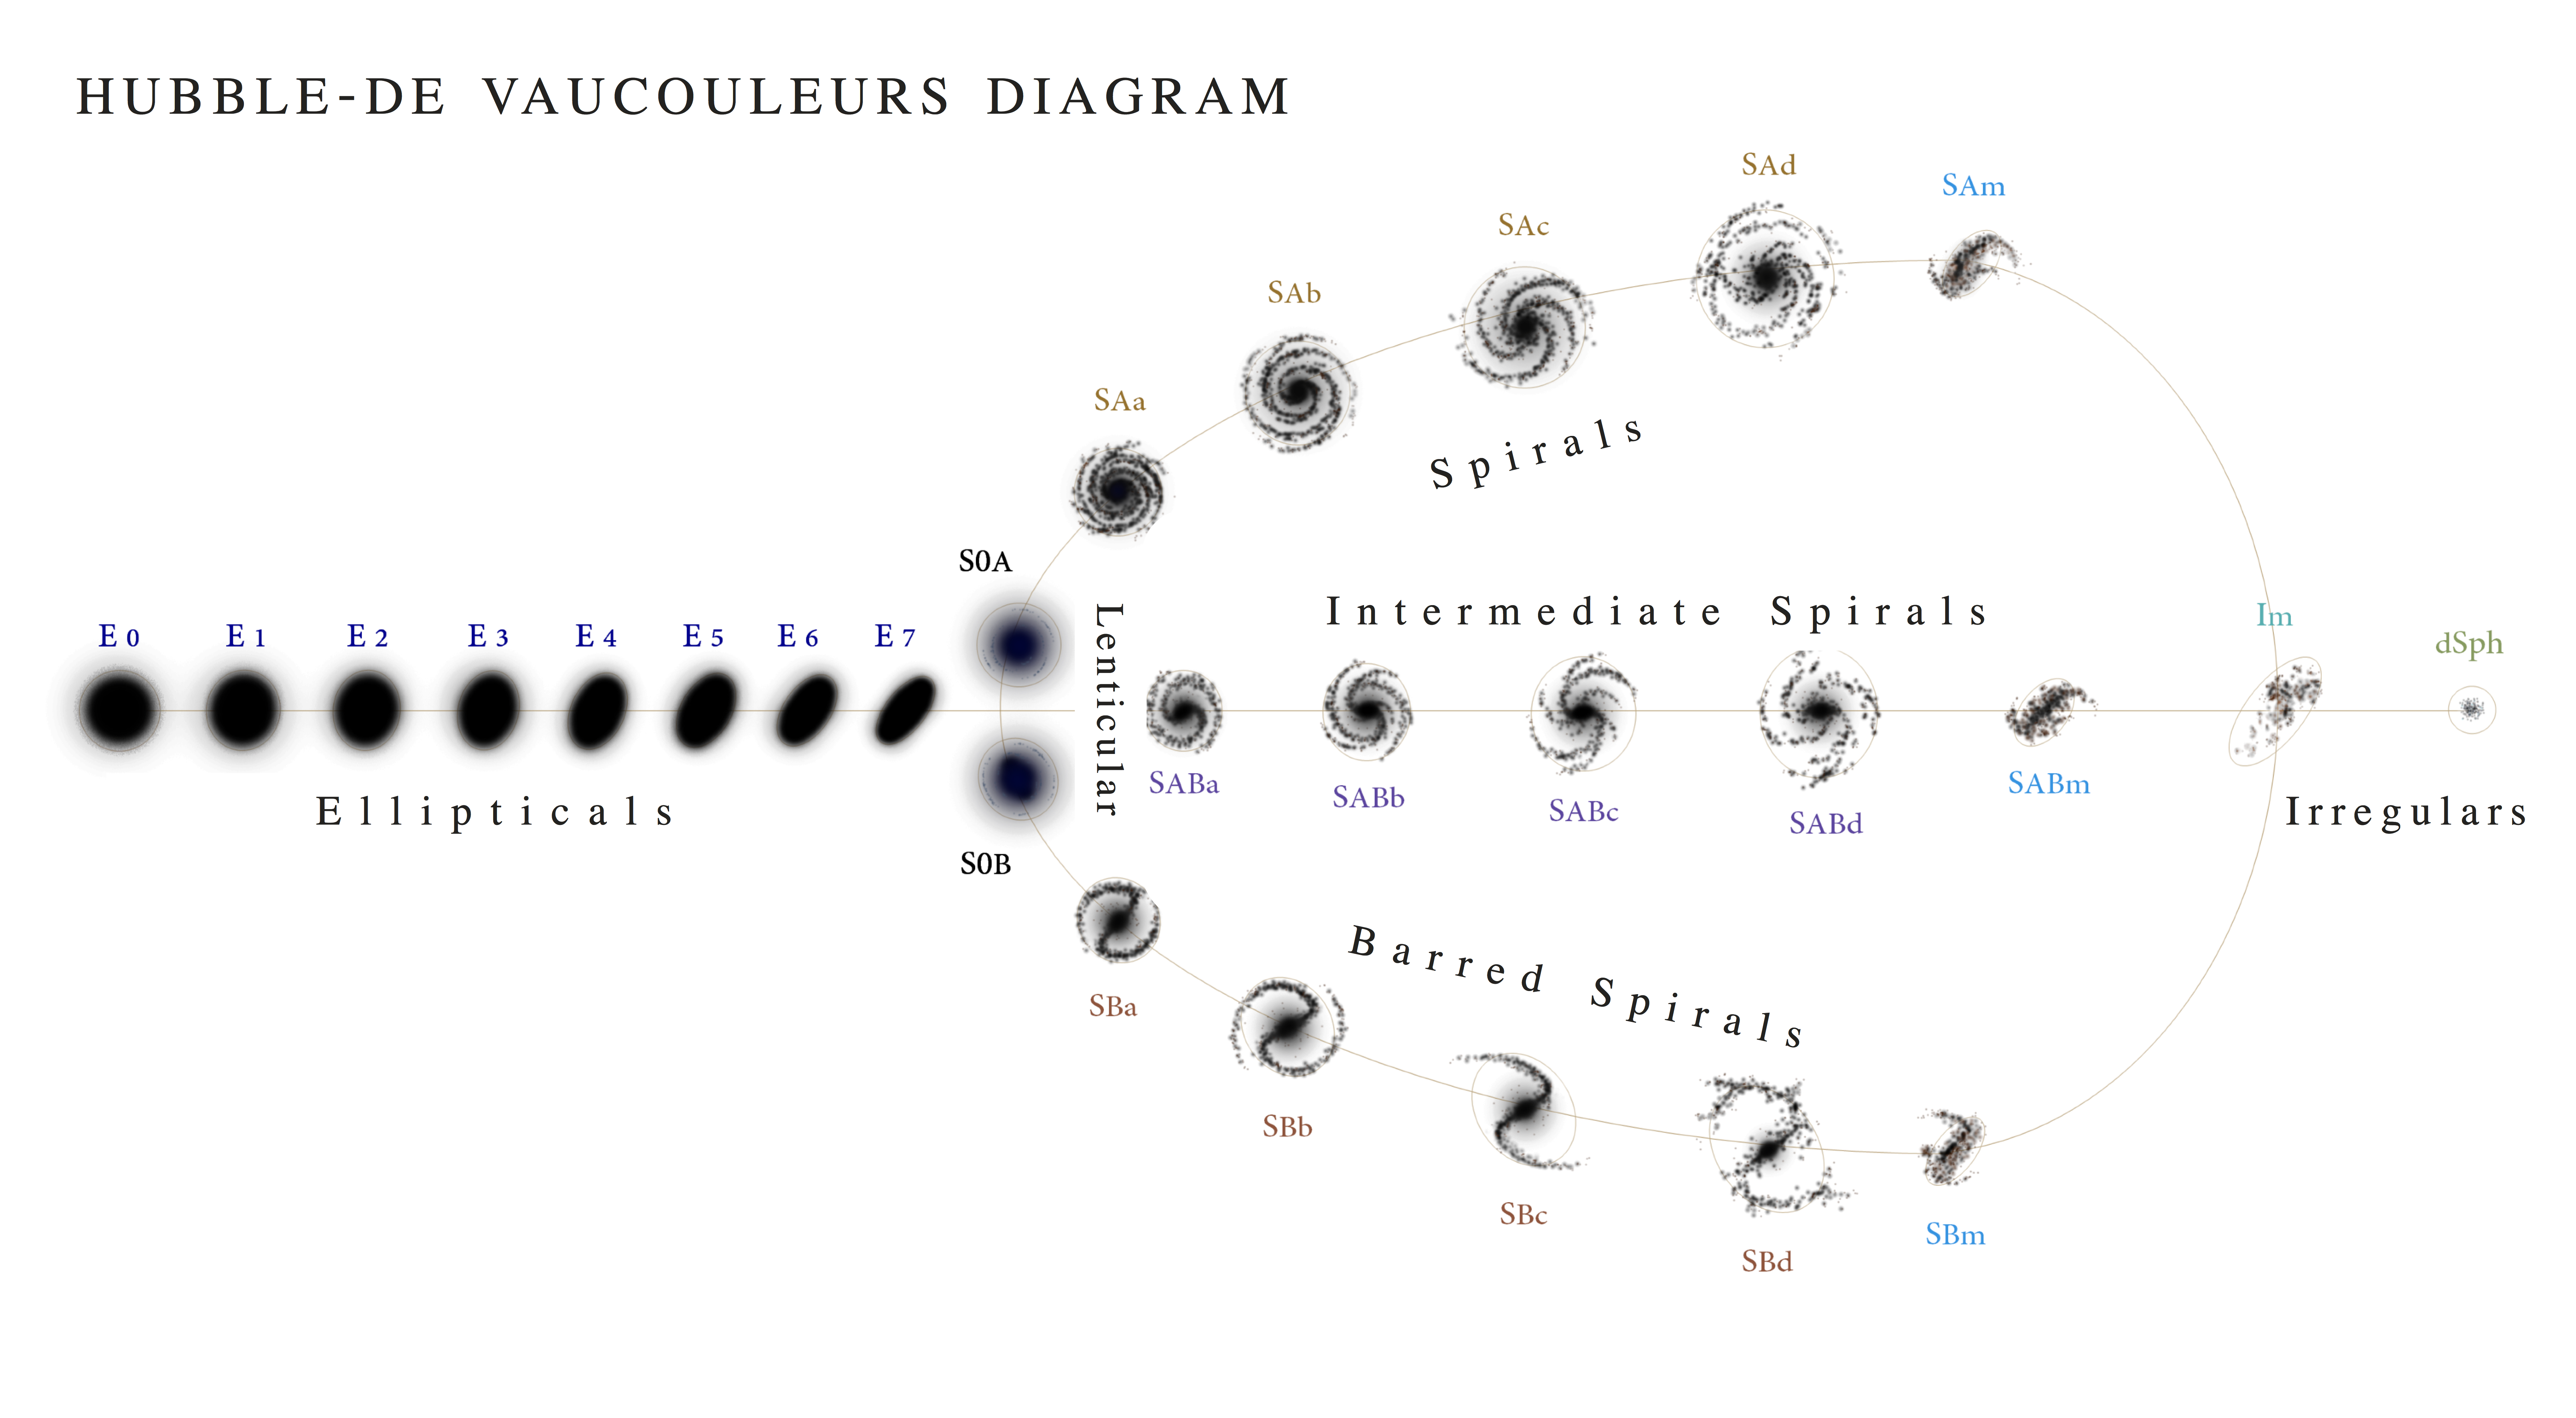
\includegraphics[width=\linewidth]{GalaxyClassificationChart}
	\caption{Hubble-de Vaucouleurs diagram for galaxy morphology.}
	\label{fig:classDiagram}
\end{figure}

Since their discovery, many various types of galaxies have been discovered and categorized into three groups (Figure \ref{fig:classDiagram}\footnote{https://commons.wikimedia.org/wiki/File:Hubble\_-\_de\_Vaucouleurs\_Galaxy\_Morphology\_Diagram.png}).

\subsection{\sc Elliptical Galaxies}

\cite{sag} Describes elliptical galaxies as round or elliptical with no visible gas and dust and lacking hot bright stars. These galaxies classified from E0 to E7 based on how elliptical they are.

\subsection{\sc Spiral Galaxies}

Spiral galaxies are the most popular of the classifications of galaxies, and also the most pleasing to the eye. They consist of a disk and spiral arms extruding from their center. Spiral galaxies have some extremely unique characteristics, the least of which are their spiral arms from which they derive their name. A sub-class of spiral galaxy known as the \textit{Barred Spiral Galaxy} is called so because of the presence of a uniquely inherited bar at their center from which their spiral arms protrude.

\subsection{\sc Irregular Galaxies}

Not quite belonging to either the spiral nor the elliptical classes of galaxies, \textit{Irregular Galaxies} are collections of gas and dust with no real structure or shape. An example of irregular galaxies in our own relative backyard would be the Magellanic Clouds. The Small and Large Magellanic Clouds have virtually no proper geometric structure and are interacting gravitationally with our own Milky Way.

\section{\sc Active Galaxies}

Thanks to advances in technology, such as the radio and X-Ray telescopes, modern astronomers and physicists have identified a new type of galaxy, the \textit{Active Galaxy}. Active galaxies are galaxies who are theorized to have an actively accreting supermassive black hole at their center. This accretion by the central black hole generates immense amounts of energy across the electromagnetic spectrum. This central black hole and its accompanying accretion disc are known as the nucleus of an active galaxy and are referred to as Active Galactic Nuclei(AGN).

\begin{figure}
	\centering
	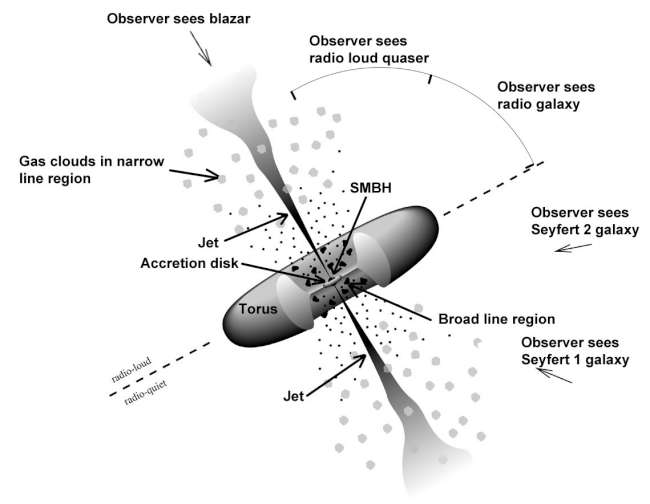
\includegraphics[width=0.6\linewidth]{UnifiedModel}
	\caption{Unified model of Active Galactic Nuclei(AGN).}
	\label{fig:unifiedModel}
\end{figure}

\subsection{\sc The Unified Model}

In order to help understand what we observe and to help produce new methods of observing AGN, the unified model was developed (Figure \ref{fig:unifiedModel}\footnote{https://fermi.gsfc.nasa.gov/science/eteu/agn/figure1.jpg}). 

In the unified model the nucleus of the active galaxy consists of a supermassive black hole surrounded by a torus of dust and gas from which it is accreting through an accretion disc formed by the gravitational pull of the supermassive black hole. Since there are a number of different types of active galaxies that have been observed, in the unified model this is described by and viewing angle to the galaxy that the observer has. For instance if an observer is viewing an active galaxy from close to edge-on, then they will see either a radio galaxy or a Seyfert 2 AGN. If however they are observing from a higher angle, then the observer will see a quasar or a Seyfert 1 depending on whether the object is radio loud or not. And finally observing from an angle equivalent to directly above will result in the observer viewing a blazar.

\section{\sc Black Holes}

Astronomical description of black holes and super-massive black holes.


\section{\sc How AGN are Observed}

\subsection{\sc Orbital X-Ray telescopes}

A description of the orbital observatories used and the bands of the EM spectrum they can observe

\newpage

\section{\sc Expected achievements}

What is expected to be achieved from this project

\newpage

\chapter{\sc The General Relativistic Description}

\section{\sc General Relativity}

An introduction to general relativity and its relation to black holes.

\subsection{\sc An introduction to Tensors}

An introduction to tensors and their mathematical properties

\subsection{\sc The Metric Tensor}

Role of the metric tensor

\subsection{\sc The Spacetime Interval}

Role of the spacetime interval

\section{\sc The Kerr Spinning Black Hole}

Description of the concept of the Kerr spinning black hole and its importance.

\subsection{\sc The Kerr Solution}

The mathematics of the Kerr solution.

\subsection{\sc Properties of the Kerr Solution}

Properties of the Kerr solution.

\chapter{\sc Statistical Analysis}

\section{\sc The Structure Function}

\citep{collier2001}
What the structure function is and how it applies to this data sample. Why it was chosen.

\section{\sc The Data}

An overview of the data. This section will contain many figures.

\chapter{\sc Programming SFA}

\section{\sc SFA usage and description}

A description of what SFA was developed for and its usage.

\section{\sc The SFA algorithm}

\subsection{\sc Process}

The logical process SFA follows to generate the structure function

\subsection{\sc Cost and Complexity}

An overview of the general running cost and Big-Oh order of SFA

\section{\sc Expected Output}

What one should expect for results from running SFA

\chapter{\sc Results and Conclusions}

\section{\sc Results}

A review of the results of running SFA on observational data

\section{\sc Conclusions}

Theoretical conclusions based on the findings of SFA

\chapter{\sc Future Work}

Potential future work and applications of SFA


\appendix

\chapter{SFA}
\label{app:sfa}
If you wanted an appendix, it would go in like this.  It would be 
referenced using Appendix~\ref{app:sfa}.


\begin{singlespace}
\bibliography{SMU-HonorsThesis-template}
\end{singlespace}
\end{document}
